% ============================================================
%  Chemistry DPP — JEE Advanced 2026 | Class 12 | SolveFlow
% ============================================================
\documentclass[12pt,a4paper]{article}

\usepackage[a4paper, margin=2cm, top=2.5cm, bottom=2.5cm]{geometry}
\usepackage{xcolor}
\usepackage[most,breakable]{tcolorbox}
\usepackage{tikz}
\usepackage{amsmath,amssymb}
\usepackage{booktabs}
\usepackage{colortbl}
\usepackage{fancyhdr}
\usepackage{enumitem}
\usepackage{array}
\usepackage{multicol}
\usepackage{lastpage}

\usetikzlibrary{shapes.geometric,arrows.meta,positioning,calc,decorations.pathreplacing}

% ── Colours ──────────────────────────────────────────────────
\definecolor{accentcolor}{HTML}{6A1B9A}
\definecolor{accentlight}{HTML}{F3E5F5}
\definecolor{questionbg}{HTML}{F3E5F5}
\definecolor{questionborder}{HTML}{6A1B9A}
\definecolor{answerbg}{HTML}{E8F5E9}
\definecolor{answerborder}{HTML}{2E7D32}
\definecolor{notebg}{HTML}{FFF3E0}
\definecolor{noteborder}{HTML}{E65100}
\definecolor{rowA}{HTML}{F5F5F5}
\definecolor{rowB}{HTML}{FFFFFF}
\definecolor{darktext}{HTML}{212121}
\definecolor{mutedtext}{HTML}{757575}
\definecolor{coverdark}{HTML}{4A148C}

% ── tcolorbox environments ────────────────────────────────────
\tcbuselibrary{skins,breakable,theorems}

\newtcolorbox{questionbox}[4]{
  enhanced, breakable,
  colback=questionbg, colframe=questionborder,
  boxrule=1pt, arc=4pt,
  title={\textbf{Q#1}\quad\textbar\quad\textit{#2}\hfill Marks:\ \textbf{#3}\quad\textbar\quad CO/BL:\ #4},
  fonttitle=\small\bfseries\color{white},
  colbacktitle=accentcolor,
  attach boxed title to top left={yshift=-2mm,xshift=4mm},
  boxed title style={arc=3pt,colframe=accentcolor},
  top=6mm
}

% ── Header / Footer ──────────────────────────────────────────
\pagestyle{fancy}
\fancyhf{}
\fancyhead[L]{\small\color{accentcolor}\textbf{Chemistry DPP \#1}}
\fancyhead[C]{\small\color{darktext}JEE Advanced 2026 \ $\cdot$\ Class 12}
\fancyhead[R]{\small\color{accentcolor}\textbf{SolveFlow}}
\fancyfoot[L]{\small\color{mutedtext}Topics: Electrochemistry, Kinetics, p-Block, d-Block, Coordination, Organic}
\fancyfoot[C]{\small Page \thepage\ of \pageref{LastPage}}
\fancyfoot[R]{\small\color{mutedtext}Marks: +4 / $-$1}
\renewcommand{\headrulewidth}{0.6pt}
\renewcommand{\footrulewidth}{0.4pt}

% ── mhchem not available — define simple arrow ───────────────
\newcommand{\yields}{\;\longrightarrow\;}
\newcommand{\equil}{\;\rightleftharpoons\;}

% ─────────────────────────────────────────────────────────────
\begin{document}

% ═══════════════════════════════════════════════════════════
%  COVER PAGE
% ═══════════════════════════════════════════════════════════
\thispagestyle{empty}

\begin{tikzpicture}[remember picture, overlay]
  \fill[coverdark] (current page.north west) rectangle ([yshift=-4.2cm]current page.north east);
  \fill[accentcolor] ([yshift=-4.2cm]current page.north west) rectangle ([yshift=-4.7cm]current page.north east);
\end{tikzpicture}

\vspace*{0.4cm}
{\color{white}\fontsize{28}{34}\selectfont\bfseries\hspace{1cm}Chemistry}\\[4pt]
{\color{white!80!black}\fontsize{14}{18}\selectfont\hspace{1cm}Daily Practice Paper \#1\quad$\cdot$\quad JEE Advanced 2026\quad$\cdot$\quad Class 12}\\[2pt]
{\color{white!60!black}\fontsize{11}{14}\selectfont\hspace{1cm}SolveFlow\quad$\cdot$\quad Demo Paper}

\vspace{2.2cm}

\begin{center}
\renewcommand{\arraystretch}{1.4}
\begin{tabular}{>{\bfseries\color{accentcolor}}p{5cm} p{8cm}}
\toprule
\rowcolor{rowA} Field & Value \\
\midrule
\rowcolor{rowB} Subject & Chemistry \\
\rowcolor{rowA} Total Questions & 10 \\
\rowcolor{rowB} Total Marks & 40 \\
\rowcolor{rowA} Negative Marking & $-1$ per wrong answer \\
\rowcolor{rowB} Time Suggested & 30 minutes \\
\rowcolor{rowA} Syllabus & Class 12 — Electrochemistry, Kinetics, \\
         & p-Block, d-Block, Coordination, Organic \\
\bottomrule
\end{tabular}
\end{center}

\vspace{0.6cm}

\begin{center}
{\color{accentcolor}\large\bfseries CO \& Bloom's Level Mapping}\\[6pt]
\renewcommand{\arraystretch}{1.35}
\begin{tabular}{>{\centering\arraybackslash}p{1.2cm}
                >{\raggedright\arraybackslash}p{5cm}
                >{\centering\arraybackslash}p{1.5cm}
                >{\raggedright\arraybackslash}p{4cm}}
\toprule
\rowcolor{accentcolor}
\color{white}\bfseries Q No. & \color{white}\bfseries Topic & \color{white}\bfseries CO & \color{white}\bfseries Bloom's Level \\
\midrule
\rowcolor{rowB} 1  & Electrochemistry — Daniell Cell      & CO1 & L3 — Apply \\
\rowcolor{rowA} 2  & Chemical Kinetics — First Order       & CO1 & L3 — Apply \\
\rowcolor{rowB} 3  & Surface Chemistry — Adsorption        & CO2 & L2 — Understand \\
\rowcolor{rowA} 4  & p-Block — Bond Angles                 & CO2 & L4 — Analyse \\
\rowcolor{rowB} 5  & d-Block — Oxidation States            & CO3 & L2 — Understand \\
\rowcolor{rowA} 6  & Coordination Chemistry — IUPAC        & CO3 & L3 — Apply \\
\rowcolor{rowB} 7  & Aldehydes \& Ketones — Tollens'       & CO4 & L4 — Analyse \\
\rowcolor{rowA} 8  & Amines — Basic Strength               & CO4 & L4 — Analyse \\
\rowcolor{rowB} 9  & Polymers — Nylon-6,6                  & CO5 & L1 — Remember \\
\rowcolor{rowA} 10 & Biomolecules — Protein Structure      & CO5 & L2 — Understand \\
\bottomrule
\end{tabular}
\end{center}

\vspace{0.6cm}

\begin{tcolorbox}[colback=accentlight,colframe=accentcolor,arc=4pt,boxrule=1pt,
  title={\bfseries\color{white} Instructions},colbacktitle=accentcolor]
\begin{itemize}[noitemsep,topsep=2pt]
  \item Each question carries \textbf{4 marks} for a correct answer.
  \item \textbf{$-1$ mark} is deducted for each incorrect answer.
  \item No marks are deducted for unattempted questions.
  \item Use of calculator is \textbf{not} permitted.
  \item All reactions assumed to occur in aqueous solution unless stated otherwise.
\end{itemize}
\end{tcolorbox}

\newpage

% ═══════════════════════════════════════════════════════════
%  QUESTIONS
% ═══════════════════════════════════════════════════════════

% ── Q1 ───────────────────────────────────────────────────────
\begin{questionbox}{1}{Electrochemistry — Daniell Cell}{4}{CO1 / L3}
The standard electrode potentials are: $E^\circ(\text{Zn}^{2+}/\text{Zn}) = -0.76\,\text{V}$
and $E^\circ(\text{Cu}^{2+}/\text{Cu}) = +0.34\,\text{V}$.
The EMF of the Daniell cell
$\text{Zn}\,|\,\text{ZnSO}_4\,||\,\text{CuSO}_4\,|\,\text{Cu}$
under standard conditions is:

\begin{center}
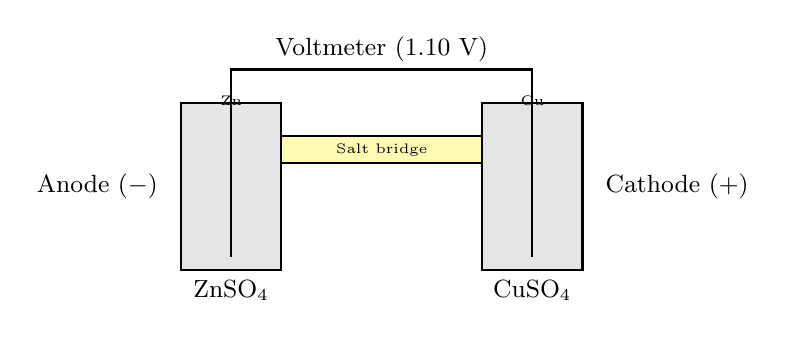
\begin{tikzpicture}[scale=0.85, font=\small]
  % Zn half-cell
  \draw[thick,fill=gray!20] (-3,-1) rectangle (-1.5,1.5);
  \draw[thick,fill=blue!60!black] (-2.25,-0.8)--(-2.25,1.3) node[above]{\tiny Zn};
  \node at (-2.25,-1.3) {ZnSO$_4$};
  % Cu half-cell
  \draw[thick,fill=gray!20] (1.5,-1) rectangle (3,1.5);
  \draw[thick,fill=orange!80!black] (2.25,-0.8)--(2.25,1.3) node[above]{\tiny Cu};
  \node at (2.25,-1.3) {CuSO$_4$};
  % Salt bridge
  \draw[thick,fill=yellow!30] (-1.5,0.6) rectangle (1.5,1.0);
  \node at (0,0.8) {\tiny Salt bridge};
  % External circuit
  \draw[thick] (-2.25,1.3)--(-2.25,2.0)--(2.25,2.0)--(2.25,1.3);
  \node at (0,2.3) {Voltmeter (1.10 V)};
  % Labels
  \node[left] at (-3.2,0.25) {\small Anode ($-$)};
  \node[right] at (3.2,0.25) {\small Cathode ($+$)};
\end{tikzpicture}
\end{center}

\begin{enumerate}[label=(\Alph*), itemsep=4pt, topsep=6pt]
  \item $-1.10\,\text{V}$
  \item $+1.10\,\text{V}$
  \item $+0.42\,\text{V}$
  \item $-0.42\,\text{V}$
\end{enumerate}
\end{questionbox}




% ── Q2 ───────────────────────────────────────────────────────
\begin{questionbox}{2}{Chemical Kinetics — First Order Reaction}{4}{CO1 / L3}
For a first-order reaction, the half-life $t_{1/2} = 693\,\text{s}$.
The rate constant $k$ is:

\begin{enumerate}[label=(\Alph*), itemsep=4pt, topsep=6pt]
  \item $1.0 \times 10^{-3}\,\text{s}^{-1}$
  \item $0.693\,\text{s}^{-1}$
  \item $1.0 \times 10^{-2}\,\text{s}^{-1}$
  \item $693\,\text{s}^{-1}$
\end{enumerate}
\end{questionbox}




% ── Q3 ───────────────────────────────────────────────────────
\begin{questionbox}{3}{Surface Chemistry — Physisorption vs Chemisorption}{4}{CO2 / L2}
Physisorption differs from chemisorption primarily because physisorption:

\begin{enumerate}[label=(\Alph*), itemsep=4pt, topsep=6pt]
  \item Involves high activation energy
  \item Is highly specific to the adsorbent
  \item Is reversible and involves van der Waals forces
  \item Forms covalent bonds with the surface
\end{enumerate}
\end{questionbox}




% ── Q4 ───────────────────────────────────────────────────────
\begin{questionbox}{4}{p-Block Elements — Bond Angles}{4}{CO2 / L4}
The correct order of bond angles among $\text{NH}_3$, $\text{NF}_3$, and $\text{PH}_3$ is:

\begin{enumerate}[label=(\Alph*), itemsep=4pt, topsep=6pt]
  \item $\text{NH}_3 > \text{NF}_3 > \text{PH}_3$
  \item $\text{NF}_3 > \text{NH}_3 > \text{PH}_3$
  \item $\text{NH}_3 > \text{PH}_3 > \text{NF}_3$
  \item $\text{PH}_3 > \text{NH}_3 > \text{NF}_3$
\end{enumerate}
\end{questionbox}




% ── Q5 ───────────────────────────────────────────────────────
\begin{questionbox}{5}{d-Block Elements — Manganese Oxoanions}{4}{CO3 / L2}
The highest oxidation state of Mn in its common oxoanion is $+7$.
The formula of the \textbf{permanganate ion} is:

\begin{enumerate}[label=(\Alph*), itemsep=4pt, topsep=6pt]
  \item $\text{MnO}_4^-$
  \item $\text{MnO}_4^{2-}$
  \item $\text{Mn}_2\text{O}_7$
  \item $\text{MnO}_2$
\end{enumerate}
\end{questionbox}




% ── Q6 ───────────────────────────────────────────────────────
\begin{questionbox}{6}{Coordination Chemistry — IUPAC Nomenclature}{4}{CO3 / L3}
The IUPAC name of $[\text{Co}(\text{NH}_3)_4(\text{NO}_2)\text{Cl}]\text{Cl}$ is:

\begin{enumerate}[label=(\Alph*), itemsep=4pt, topsep=6pt]
  \item Tetraamminechloronitrocobalt(III) chloride
  \item Tetraamminechloridonitrito-$\kappa O$-cobalt(III) chloride
  \item Tetraamminenitrochloridocobalt(III) chloride
  \item Chloridotetraamminenitroso-cobalt(III) chloride
\end{enumerate}
\end{questionbox}




% ── Q7 ───────────────────────────────────────────────────────
\begin{questionbox}{7}{Aldehydes \& Ketones — Tollens' vs Fehling's Test}{4}{CO4 / L4}
Which compound gives a \textbf{positive Tollens' test} but \textbf{negative Fehling's test}?

\begin{enumerate}[label=(\Alph*), itemsep=4pt, topsep=6pt]
  \item Formaldehyde (HCHO)
  \item Acetaldehyde (CH$_3$CHO)
  \item Benzaldehyde (C$_6$H$_5$CHO)
  \item Acetone (CH$_3$COCH$_3$)
\end{enumerate}
\end{questionbox}




% ── Q8 ───────────────────────────────────────────────────────
\begin{questionbox}{8}{Amines — Basic Strength in Aqueous Solution}{4}{CO4 / L4}
The correct order of basic strength of amines \textbf{in aqueous solution} is:

\begin{enumerate}[label=(\Alph*), itemsep=4pt, topsep=6pt]
  \item $(CH_3)_3N > (CH_3)_2NH > CH_3NH_2 > NH_3$
  \item $(CH_3)_2NH > CH_3NH_2 > (CH_3)_3N > NH_3$
  \item $CH_3NH_2 > (CH_3)_2NH > (CH_3)_3N > NH_3$
  \item $NH_3 > CH_3NH_2 > (CH_3)_2NH > (CH_3)_3N$
\end{enumerate}
\end{questionbox}




% ── Q9 ───────────────────────────────────────────────────────
\begin{questionbox}{9}{Polymers — Nylon-6,6}{4}{CO5 / L1}
Nylon-6,6 is formed by the condensation polymerisation of:

\begin{enumerate}[label=(\Alph*), itemsep=4pt, topsep=6pt]
  \item Caprolactam
  \item Hexamethylenediamine and adipic acid
  \item Hexamethylenediamine and sebacic acid
  \item Glycol and terephthalic acid
\end{enumerate}
\end{questionbox}




% ── Q10 ──────────────────────────────────────────────────────
\begin{questionbox}{10}{Biomolecules — Protein Secondary Structure}{4}{CO5 / L2}
The secondary structure of a protein is maintained primarily by:

\begin{enumerate}[label=(\Alph*), itemsep=4pt, topsep=6pt]
  \item Peptide bonds ($-$CO$-$NH$-$)
  \item Disulfide bridges ($-$S$-$S$-$)
  \item Hydrogen bonds between C$=$O and N$-$H groups of the backbone
  \item Ionic interactions between charged side chains
\end{enumerate}
\end{questionbox}



\label{LastPage}
\end{document}
